\documentclass[14pt, a4paper]{extarticle}
\usepackage[T2A]{fontenc}
\usepackage[utf8]{inputenc}
\usepackage[english,russian]{babel}
\usepackage[left = 3cm, right = 1cm, top = 2cm, bottom = 2cm]{geometry}
\setlength\parindent{12.5mm} 
\linespread{1.3}
\usepackage{enumitem}
\usepackage{amsmath}
\usepackage{amssymb}
\usepackage{wrapfig}
\usepackage{indentfirst}
\usepackage{hyperref} % ДОЛЖЕН БЫТЬ ПОСЛЕДНИМ (кроме cleveref)
\hypersetup{
	colorlinks=true,
	citecolor=blue,
	urlcolor=blue, 
	linkcolor=blue,
	pdfencoding=auto
}
\usepackage{xcolor}   % Пакет для работы с цветами
\usepackage{listings} % Пакет для оформления кода
\usepackage{graphicx}
\usepackage{float}
\usepackage{longtable}
\usepackage[htt]{hyphenat}
% Определяем приглушенные цвета для академического стиля
\definecolor{codegreen}{rgb}{0,0.6,0}
\definecolor{codegray}{rgb}{0.5,0.5,0.5}
\definecolor{codepurple}{rgb}{0.58,0,0.82}
\definecolor{backcolour}{rgb}{0.97,0.97,0.97}
% Глобальная настройка стиля листингов
\lstset{ 
	language=C++,                       % Указываем язык по умолчанию
	backgroundcolor=\color{backcolour}, % Светло-серый фон
	commentstyle=\color{codegreen}\itshape, % Комментарии зеленым курсивом
	keywordstyle=\color{blue}\bfseries, % Ключевые слова синим и жирным
	numberstyle=\tiny\color{codegray},  % Стиль номеров строк (мелкий, серый)
	stringstyle=\color{codepurple},     % Строки фиолетовым
	basicstyle=\ttfamily\footnotesize,  % Моноширинный шрифт, чуть меньше основного
	breakatwhitespace=false,         
	breaklines=true,                    % Автоматический перенос длинных строк
	captionpos=t,                       % Позиция заголовка (t - сверху, b - снизу)
	keepspaces=true,                 
	numbers=left,                       % Номера строк слева
	numbersep=10pt,                     % Отступ номеров от кода
	showspaces=false,                
	showstringspaces=false,
	showtabs=false,                  
	tabsize=4,                          % Размер табуляции
	frame=single,                       % Одинарная рамка вокруг кода
	rulecolor=\color{black!30},          % Цвет рамки (светло-серый)
	extendedchars=\true
}
\newcommand{\tab}{\hspace{12.5mm}}

\usepackage{tabularx} % Обязательный пакет для этого способа

% Создаем команду для удобного центрирования текста внутри растягиваемых ячеек
\newcolumntype{Y}{>{\centering\arraybackslash}X}

\begin{document}
\thispagestyle{empty}
\begin{center}
    \hspace{0.2cm}МИНИСТЕРСТВО НАУКИ И ВЫСШЕГО ОБРАЗОВАНИЯ РОССИЙСКОЙ ФЕДЕРАЦИИ\\
    Федеральное государственное автономное образовательное\\
    учреждение высшего образования\\
    {\bf <<Санкт-Петербургский политехнический\\
    университет Петра Великого>>}\\
    Институт компьютерных наук и кибербезопасности\\
    Высшая школа технологий искусственного интеллекта\\
    02.03.01\_03 Технологии машинного обучения и искусственного интеллекта\\
    \vspace{3cm}
    \Large\bf{
        Отчёт о выполнении лабораторной работы №4\\
        Основы архитектуры ЦВМ\\[1cm]
    }
\end{center}
\vspace{2cm}
\begin{flushleft}
    {\bf Выполнил:}\\
    Cтудент группы 5130201/50302 \hfill
    \line(1,0){4cm} \quad Калинский В.И.\\
    {\bf Принял:}\\
    К.т.н., доцент, доцент ВШТИИ и КОЦ ИИ \hfill
    \line(1,0){3 cm} \quad Вербова Н.М.\\[0.5cm]
    { \hfill<<\rule{1cm}{0.5pt}>>\rule{2cm}{0.5pt}\hspace{3pt}2026 г.}
\end{flushleft}
\vspace{1cm}
\begin{center}
    Санкт-Петербург, 2026
\end{center}
\newpage
\textbf{Цель работы:}

\noindent Изучить принцип работы сдвигающих регистров.
\\\\
\textbf{Методика:}

В первой части работы необходимо синтезировать последовательный (сдвигающий) 4-разрядный регистр. Для определения межтриггерных связей рассмотрим процесс передачи информации между $(i+1)$-м (предыдущим) и $i$-м (последующим) триггерами регистра при сдвиге кода числа. 

Составим таблицу переходов $i$-го триггера из состояния $Q_i^t$ (до прихода сдвигающего импульса) в состояние $Q_i^{t+1}$ (после прихода импульса) в зависимости от его собственного состояния $Q_i^t$ и состояния предыдущего триггера $Q_{i+1}^t$ (таблица \ref{tab:trans}). В качестве элементной базы выберем тактируемые $J$-$K$ триггеры.

\begin{table}[H]
	\centering
	\begin{tabular}{|c|c|c|c|c|c|}
		\hline
		$Q_{i+1}^t$ & $Q_i^t$ & $Q_i^{t+1}$ & Переход $Q_i^t \to Q_i^{t+1}$ & $J_i^t$ & $K_i^t$ \\ \hline
		0 & 0 & 0 & $0 \to 0$ & 0 & * \\ \hline
		0 & 1 & 0 & $1 \to 0$ & * & 1 \\ \hline
		1 & 0 & 1 & $0 \to 1$ & 1 & * \\ \hline
		1 & 1 & 1 & $1 \to 1$ & * & 0 \\ \hline
	\end{tabular}
	\caption{Таблица переходов и управляющих сигналов $i$-го триггера}
	\label{tab:trans}
\end{table}

На основе таблицы \ref{tab:trans} построим прикладную таблицу и карты Карно для входов $J_i$ и $K_i$. Жирным шрифтом выделены контуры склеивания.

\begin{center}
	\small
	\begin{minipage}{0.32\textwidth}
		\centering
		\textbf{$Q_i^t \to Q_i^{t+1}$}\\[4pt]
		\begin{tabular}{|c|c|c|}
			\hline
			& $Q_i^t$ & $\overline{Q}_i^t$ \\ \hline
			$Q_{i+1}^t$ & 11 & 01 \\ \hline
			$\overline{Q}_{i+1}^t$ & 10 & 00 \\ \hline
		\end{tabular}
	\end{minipage}
	\hfill
	\begin{minipage}{0.32\textwidth}
		\centering
		\textbf{$J_i$}\\[4pt]
		\begin{tabular}{|c|c|c|}
			\hline
			& $Q_i^t$ & $\overline{Q}_i^t$ \\ \hline
			$Q_{i+1}^t$ & \textbf{*} & \textbf{1} \\ \hline
			$\overline{Q}_{i+1}^t$ & * & 0 \\ \hline
		\end{tabular}
	\end{minipage}
	\hfill
	\begin{minipage}{0.32\textwidth}
		\centering
		\textbf{$K_i$}\\[4pt]
		\begin{tabular}{|c|c|c|}
			\hline
			& $Q_i^t$ & $\overline{Q}_i^t$ \\ \hline
			$Q_{i+1}^t$ & 0 & * \\ \hline
			$\overline{Q}_{i+1}^t$ & \textbf{1} & \textbf{*} \\ \hline
		\end{tabular}
	\end{minipage}
\end{center}

По результатам минимизации карт Карно получаем уравнения межтриггерных связей:
\begin{align*}
	J_i^t &= Q_{i+1}^t, & K_i^t &= \overline{Q}_{i+1}^t.
\end{align*}
Для входного (первого по ходу сдвига) триггера роль сигнала $Q_{i+1}^t$ выполняет внешний информационный вход $D_{\text{вх}}$: $J_{\text{вх}} = D_{\text{вх}}$, $K_{\text{вх}} = \overline{D}_{\text{вх}}$. Синтезированная схема 4-разрядного сдвигающего регистра приведена на рис. \ref{fig:4-1}.

\begin{figure}[H]
	\centering
	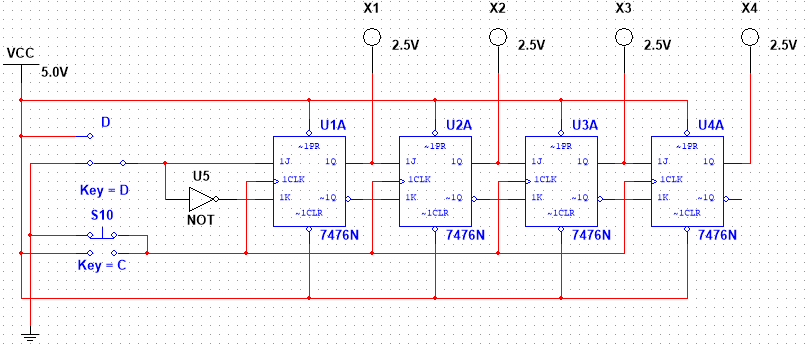
\includegraphics[width=0.75\linewidth]{4-1}
	\caption{Схема 4-разрядного последовательного сдвигового регистра}
	\label{fig:4-1}
\end{figure}

Во второй части лабораторной работы изучается принцип работы восьмиразрядного универсального сдвигового регистра ИС К155ИР13 (SN74198). Регистр позволяет выполнять параллельную загрузку данных по входам $D_1$--$D_8$, последовательный сдвиг вправо (вход $DR$, от 8-го разряда к 1-му) и сдвиг влево (вход $DL$, от 1-го разряда к 8-му) по положительному перепаду синхроимпульса на входе $C$, а также асинхронный сброс в «0» по инверсному входу $\overline{R}$ ($\text{CLR}$). Режимы работы задаются управляющими входами $S_1$ и $S_0$ согласно таблице \ref{tab:modes}.

\begin{table}[H]
	\centering
	\begin{tabular}{|c|c|c|}
		\hline
		$S_1$ & $S_0$ & Режим работы \\ \hline
		0 & 0 & Хранение \\ \hline
		0 & 1 & Сдвиг влево (от 1-го к 8-му разряду) \\ \hline
		1 & 0 & Сдвиг вправо (от 8-го к 1-му разряду) \\ \hline
		1 & 1 & Параллельная запись \\ \hline
	\end{tabular}
	\caption{Режимы работы универсального регистра К155ИР13 (SN74198)}
	\label{tab:modes}
\end{table}

На основе схемы из методических указаний (рис. \ref{fig:p4-3}) в среде Multisim была собрана схема для исследования ИС К155ИР13 (SN74198), представленная на рис. \ref{fig:4-2}.

\begin{figure}[H]
	\centering
	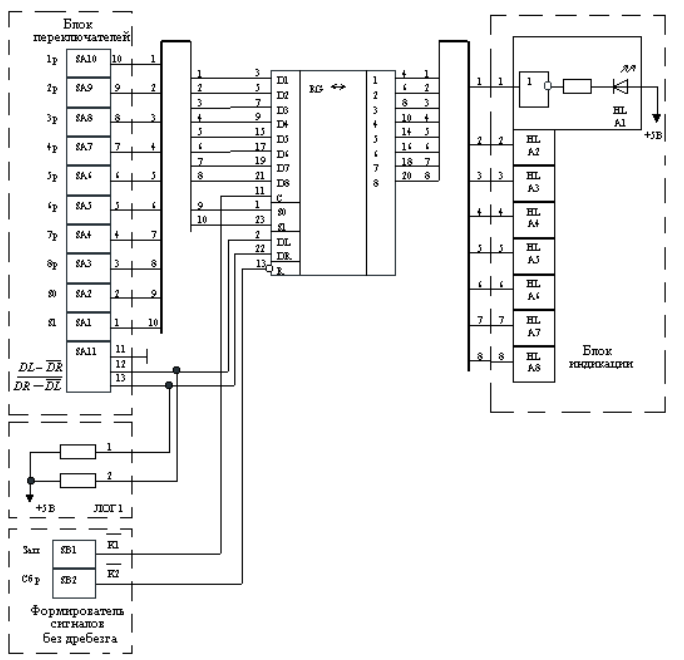
\includegraphics[width=0.7\linewidth]{p4-3}
	\caption{Принципиальная схема для исследования ИС К155ИР13 из методических указаний}
	\label{fig:p4-3}
\end{figure}

\begin{figure}[H]
	\centering
	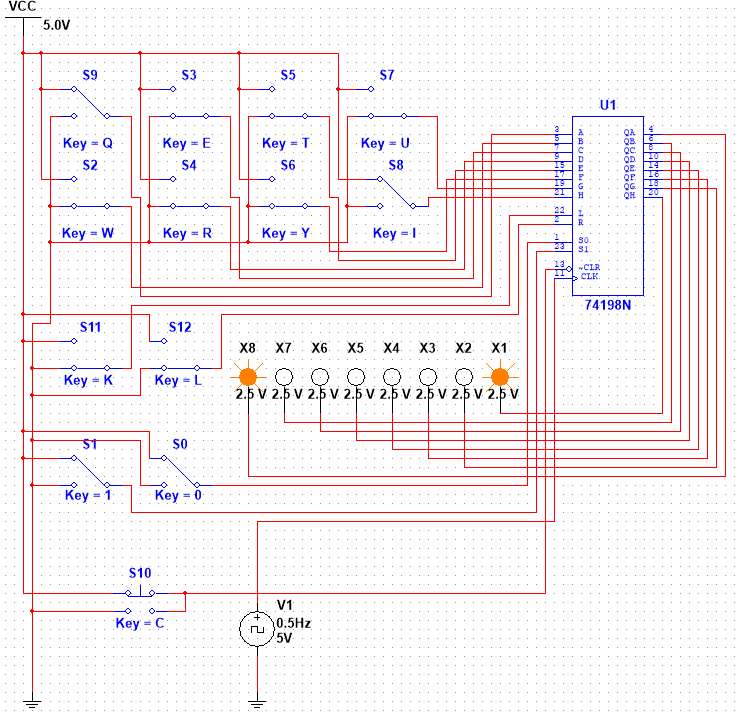
\includegraphics[width=0.75\linewidth]{4-2}
	\caption{Схема исследования регистра К155ИР13 (SN74198) в среде Multisim}
	\label{fig:4-2}
\end{figure}

В третьей части работы на базе ИС К155ИР13 (SN74198) необходимо сконструировать универсальный кольцевой сдвигающий регистр. В кольцевом регистре разряды при сдвиге не теряются, а перезаписываются с крайнего выхода в освобождающийся крайний разряд с противоположной стороны.

Для реализации циклического сдвига в обоих направлениях (как влево, так и вправо) выполним следующие соединения:
\begin{itemize}
	\item Выход старшего (8-го) разряда $Q_8$ ($Q_H$) соединяем со входом последовательного сдвига $SR$ ($DR$). При циклическом сдвиге в сторону старших разрядов бит, выходящий из 8-го разряда, возвращается на вход регистра и предотвращает опустошение разрядной сетки.
	\item Выход младшего (1-го) разряда $Q_1$ ($Q_A$) соединяем со входом последовательного сдвига $SL$ ($DL$). При сдвиге в противоположном направлении бит из 1-го разряда циклически переносится обратно в регистр, обеспечивая сохранение и непрерывную циркуляцию записанного кода.
\end{itemize}
Принципиальная схема сконструированного универсального кольцевого регистра в среде Multisim приведена на рис. \ref{fig:4-3}.

\begin{figure}[H]
	\centering
	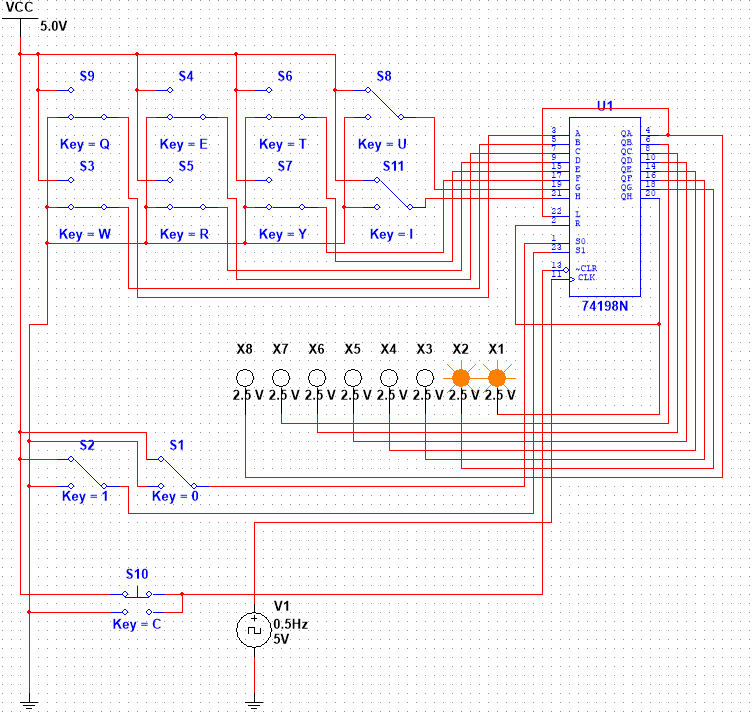
\includegraphics[width=0.75\linewidth]{4-3}
	\caption{Схема универсального кольцевого регистра на базе ИС К155ИР13 (SN74198)}
	\label{fig:4-3}
\end{figure}

\textbf{Выводы:}

В ходе выполнения лабораторной работы были изучены принципы построения и функционирования последовательных (сдвигающих) регистров. С использованием таблиц переходов и карт Карно для $J-K$ триггеров были выведены уравнения межтриггерных связей и синтезирован 4-разрядный сдвигающий регистр. Также было исследовано функционирование восьмиразрядного универсального сдвигового регистра К155ИР13 (SN74198) в режимах сброса, записи, хранения и двунаправленного сдвига. Путём замыкания цепей обратной связи между крайними выходами ($Q_1, Q_8$) и входами последовательного переноса ($DL, DR$) на базе ИС К155ИР13 был сконструирован и проверен универсальный кольцевой регистр, обеспечивающий циклический сдвиг кода числа в обоих направлениях без потери информации.

%КАРТИНКИ
%\begin{figure}[H]
%	\centering
%	\includegraphics[width=0.85\textwidth]{install_deb.png}
%	\caption{Начало установки гостевой ОС Debian 12}
%	\label{fig:vbox_setup}
%\end{figure}

%---------------------------------------------------------------------------------
%ССЫЛКИ НА САЙТ

%\href{https://www.virtualbox.org/wiki/Downloads}{официального сайта VirtualBox}

%---------------------------------------------------------------------------------
%ССЫЛКА НА ПРИЛОЖЕНИЕ

%\texttt{zlib}\cite{zlib_docs}

%---------------------------------------------------------------------------------
%ССЫЛКА НА РИСУНОК

%показано на рис. \ref{fig:vbox_setup}

%---------------------------------------------------------------------------------
%ТАБЛИЦА С ПЕРЕВОДОМ НА СЛЕДУЮЩУЮ СТРАНИЦУ

%\begin{longtable}{|l|p{0.75\textwidth}|}
%	\caption{Функции библиотеки ncurses, используемые в TUI} \label{tab:ncurses_funcs} \\
%	\hline
%	\textbf{Функция} & \textbf{Назначение и описание алгоритма работы} \\ \hline
%	\endhead
%	\texttt{initscr()} & Инициализирует библиотеку, выделяет память под внутренние структуры окна и переводит терминал ОС в графический режим. \\ \hline
%	\texttt{cbreak()} & Отключает строковую буферизацию терминала, позволяя программе мгновенно реагировать на нажатия клавиш без ожидания \texttt{Enter}. \\ \hline
%	\texttt{noecho()} & Отключает автоматический вывод (эхо) вводимых пользователем символов на экран, позволяя программе самой управлять отрисовкой. \\ \hline
%	\texttt{clear()} & Очищает виртуальный экран для подготовки к отрисовке нового кадра меню. \\ \hline
%	\texttt{move(y, x)} & Осуществляет абсолютное позиционирование курсора по координатам \texttt{Y} (строка) и \texttt{X} (столбец). \\ \hline
%	\texttt{printw()} & Аналог функции \texttt{printf} для \texttt{ncurses}: выводит отформатированный текст в текущей позиции курсора. \\ \hline
%	\texttt{getch()} & Ожидает и считывает код нажатой пользователем клавиши (включая стрелки навигации и функциональные клавиши). \\ \hline
%	\texttt{getnstr()} & Безопасно считывает строку от пользователя с аппаратным ограничением максимального количества символов (защита от переполнения). \\ \hline
%	\texttt{scanw()} & Аналог функции \texttt{scanf}, считывает форматированный ввод пользователя (применяется для ввода числовых данных). \\ \hline
%	\texttt{endwin()} & Выгружает библиотеку из памяти, восстанавливает историю команд и возвращает терминал в стандартный режим работы ОС. \\ \hline
%\end{longtable}
%---------------------------------------------------------------------------------

\end{document}